\documentclass[aspectratio=169]{beamer}

\usetheme{Madrid}
\usecolortheme{whale}
\usepackage[utf8]{inputenc}
\usepackage[T1]{fontenc}
\usepackage{booktabs}
\usepackage{graphicx}
\usepackage{amsmath,amssymb}

\graphicspath{{../figures/}}
\setbeamertemplate{navigation symbols}{}
\setbeamertemplate{footline}[frame number]
\setbeamerfont{frametitle}{size=\large}
\setbeamertemplate{section in toc}[sections numbered]

\newcommand{\act}[1]{\texttt{\small #1}}

\title[Process Mining, BPI 2013]{Process Mining and Formal Verification\\
       of the Volvo IT Incident Process}
\subtitle{BPI Challenge 2013}
\author{Francesco Sgaramella}
\date{\today}

\begin{document}

\frame{\titlepage}


\section{Context}


\begin{frame}{The question}
\begin{itemize}
  \item An IT service desk records every state change of every incident.
  \item The process is \emph{documented}. What was actually \emph{executed}?
  \bigskip
  \item Volvo IT Belgium, VINST system, 2010 to 2012.
  \item Three logs: incidents, open problems, closed problems.
  \item A standard benchmark, so the results are comparable with the literature.
  \bigskip
  \item Nothing here is read off a dashboard by eye: every figure shown is
        produced by code and pinned by a regression test.
\end{itemize}
\end{frame}

\section{The data}

\begin{frame}{The data}
\begin{center}\small\begin{tabular}{lrrrll}
\toprule
Log & Cases & Events & Activities & From & To \\
\midrule
closed\_problems & 1,487 & 6,660 & 7 & 2006-01-11 & 2012-05-31 \\
incidents & 7,554 & 65,533 & 13 & 2010-03-31 & 2012-05-22 \\
open\_problems & 819 & 2,351 & 5 & 2006-11-07 & 2012-06-15 \\
\bottomrule
\end{tabular}
\end{center}
\bigskip
\small
Case and event counts reproduce the published figures exactly, the first
check on the loader.
\bigskip

The problem logs are not variants of the incident process: median duration
differs by an order of magnitude and their alphabet is smaller. The incident log
is the object of study; the other two are used for comparison.
\end{frame}


\begin{frame}{There is no activity column}
The dataset records \act{Status} and \act{Sub Status}. What counts as an
activity is the analyst's decision.
\bigskip
\begin{columns}[T]
\begin{column}{0.48\textwidth}
\textbf{\act{Status}}: 4 activities\\[0.3em]
\act{Accepted}, \act{Queued}, \act{Completed}, \act{Unmatched}\\[0.6em]
Small models. Waiting on a vendor and waiting on a user become
indistinguishable.
\end{column}
\begin{column}{0.48\textwidth}
\textbf{\act{Status+Sub Status}}: 13 activities\\[0.3em]
\act{Accepted+In Progress}, \act{Accepted+Wait - User}, \dots\\[0.6em]
Three times larger models, lower precision, and the real process.
\end{column}
\end{columns}
\bigskip
\begin{center}
Treated as a parameter of the loader, not fixed silently. Both are reported.
\end{center}
\end{frame}


\section{Discovery}

\begin{frame}{Three discovery algorithms}
\begin{description}
  \item[Alpha] Ordering relations from directly-follows pairs. Assumes a
        complete, noise-free log. Cannot represent short loops.
  \item[Heuristics] Frequency-weighted, with a dependency threshold. Filters
        infrequent behaviour instead of modelling it. Robust to noise.
  \item[Inductive] Recursive partitioning into a process tree, converted to a
        net. Guarantees soundness and, at zero noise, perfect fitness.
\end{description}
\bigskip
All three are run on the full incident log, under both labellings, from the same
loaded bundle, so the six rows on the next slides differ only in the
algorithm and the labelling.
\end{frame}


\begin{frame}{Discovery results}
\begin{center}\scriptsize\begin{tabular}{llrrrrrr}
\toprule
Mode & Algorithm & Fitness & Precision & Gen. & Simpl. & Places & Trans. \\
\midrule
status & alpha & 0.119 & 0.400 & 0.734 & 1.000 & 2 & 4 \\
status & heuristics & 0.994 & 0.678 & 0.767 & 0.622 & 8 & 15 \\
status & inductive & 1.000 & 0.440 & 0.748 & 0.667 & 17 & 23 \\
status+substatus & alpha & 0.127 & 0.176 & 0.770 & 0.789 & 2 & 13 \\
status+substatus & heuristics & 0.948 & 0.387 & 0.634 & 0.471 & 27 & 69 \\
status+substatus & inductive & 1.000 & 0.234 & 0.783 & 0.634 & 57 & 78 \\
\bottomrule
\end{tabular}
\end{center}
\bigskip
\small
Four dimensions, and they trade off: fitness (can the model replay the log?),
precision (does it forbid what never happened?), generalisation and simplicity.
Inductive buys perfect fitness with permissiveness and the largest net.
Heuristics gives the best balance. Alpha collapses.
\bigskip

Moving from 4 labels to 13 lowers precision for every algorithm and roughly
triples the net: there is simply more distinct behaviour to explain.
\end{frame}

\begin{frame}{What the two usable miners produce}
\begin{center}
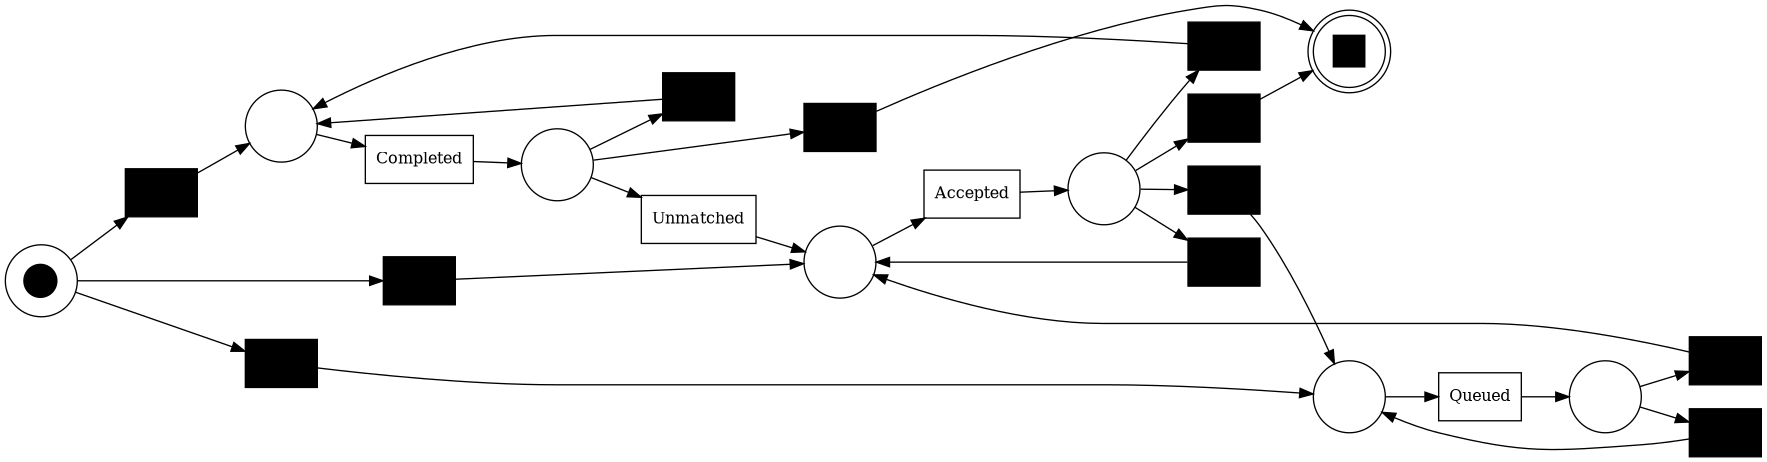
\includegraphics[width=0.66\textwidth]{petri_heuristics_status.png}\\[0.2em]
{\scriptsize Heuristics: 8 places, 15 transitions}\\[0.2em]
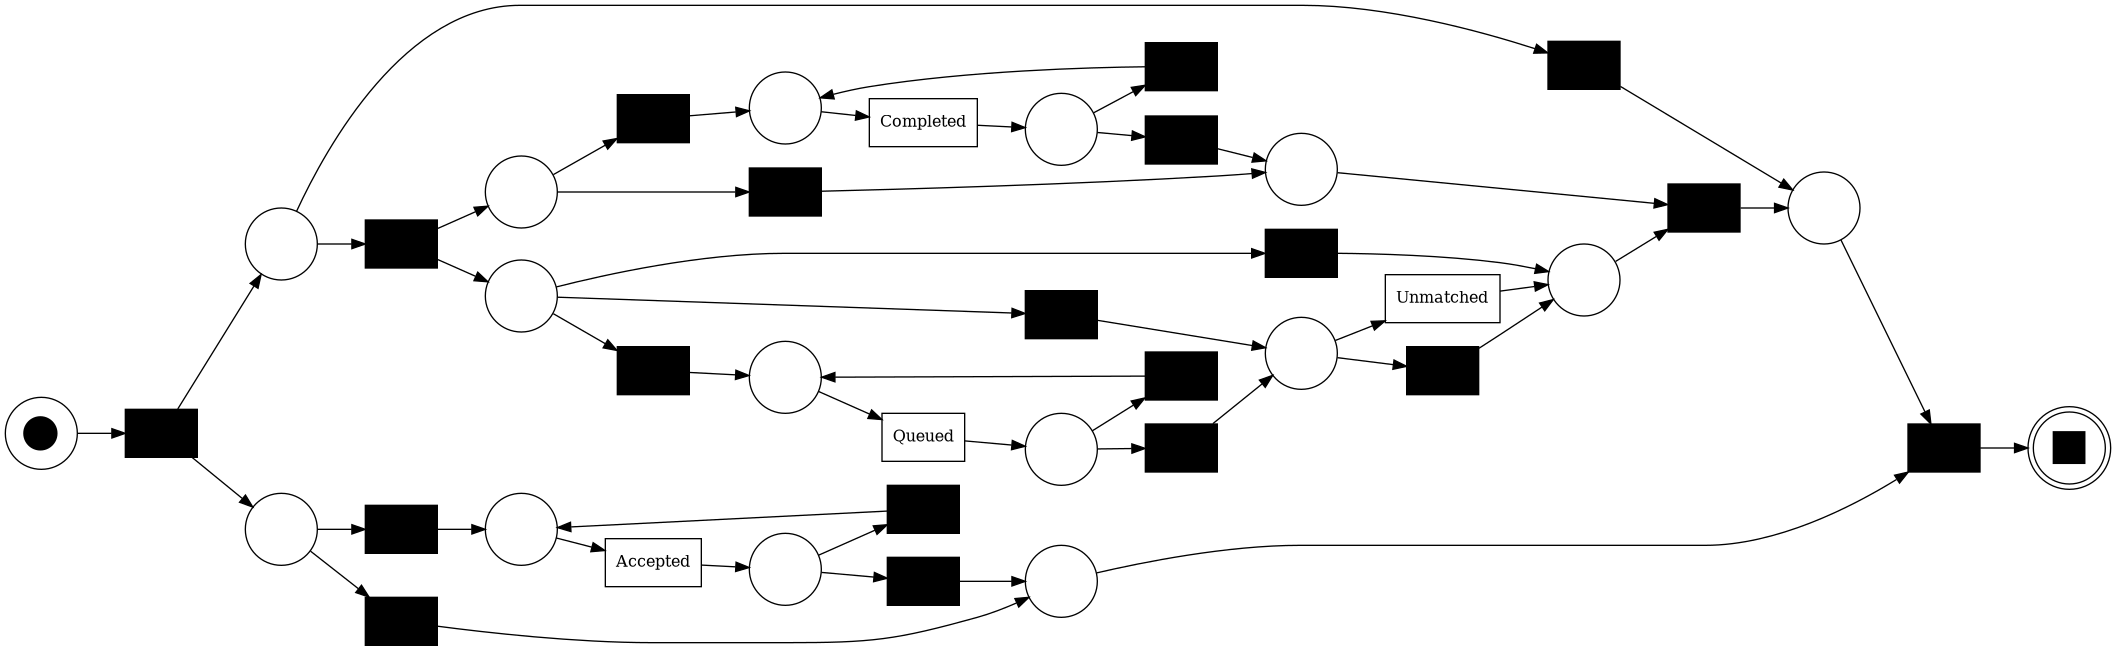
\includegraphics[width=0.66\textwidth]{petri_inductive_status.png}\\[0.2em]
{\scriptsize Inductive: 17 places, 23 transitions, plus silent routing}
\end{center}
\end{frame}


\begin{frame}{Why Alpha collapses}
\begin{columns}[T]
\begin{column}{0.55\textwidth}
Fitness below $0.15$; the net degenerates to two places.
\bigskip
\textbf{This is not a bug.}
\bigskip
90\% of cases contain a \emph{length-one loop}, an activity immediately
repeated.
\bigskip
Alpha infers contradictory ordering relations from a directly-follows pair
$(a,a)$ and provably cannot represent such loops.
\bigskip
A known theoretical boundary, demonstrated on a real log.
\end{column}
\begin{column}{0.43\textwidth}
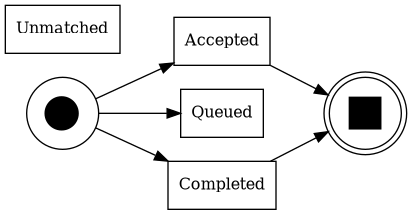
\includegraphics[width=\textwidth]{petri_alpha_status.png}
\end{column}
\end{columns}
\end{frame}

\section{Time}

\begin{frame}{Where does the time go?}
\begin{center}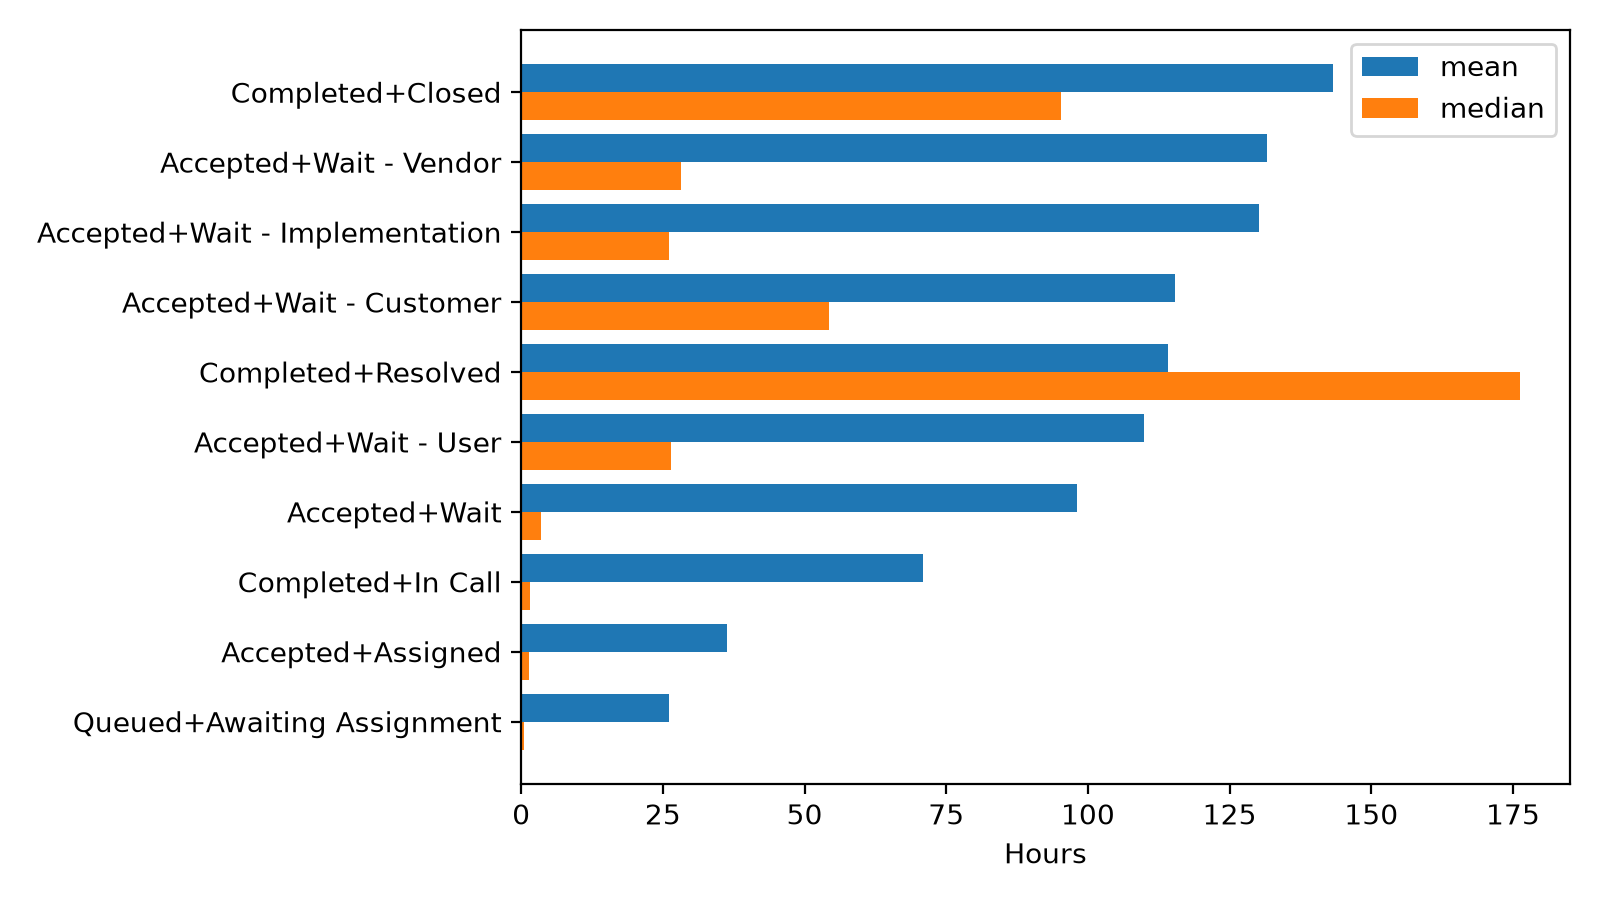
\includegraphics[width=0.66\textwidth]{waiting_times.png}\end{center}
\small
The \act{Wait} states dominate: delay is \emph{external} to the service desk.
Where mean and median diverge (\act{Accepted+In Progress} is minutes at the
median, hours at the mean) work is normally picked up at once and
occasionally stalls for months. Either figure alone misleads.
\end{frame}




\begin{frame}{A weakly standardised process}
\begin{columns}[T]
\begin{column}{0.5\textwidth}
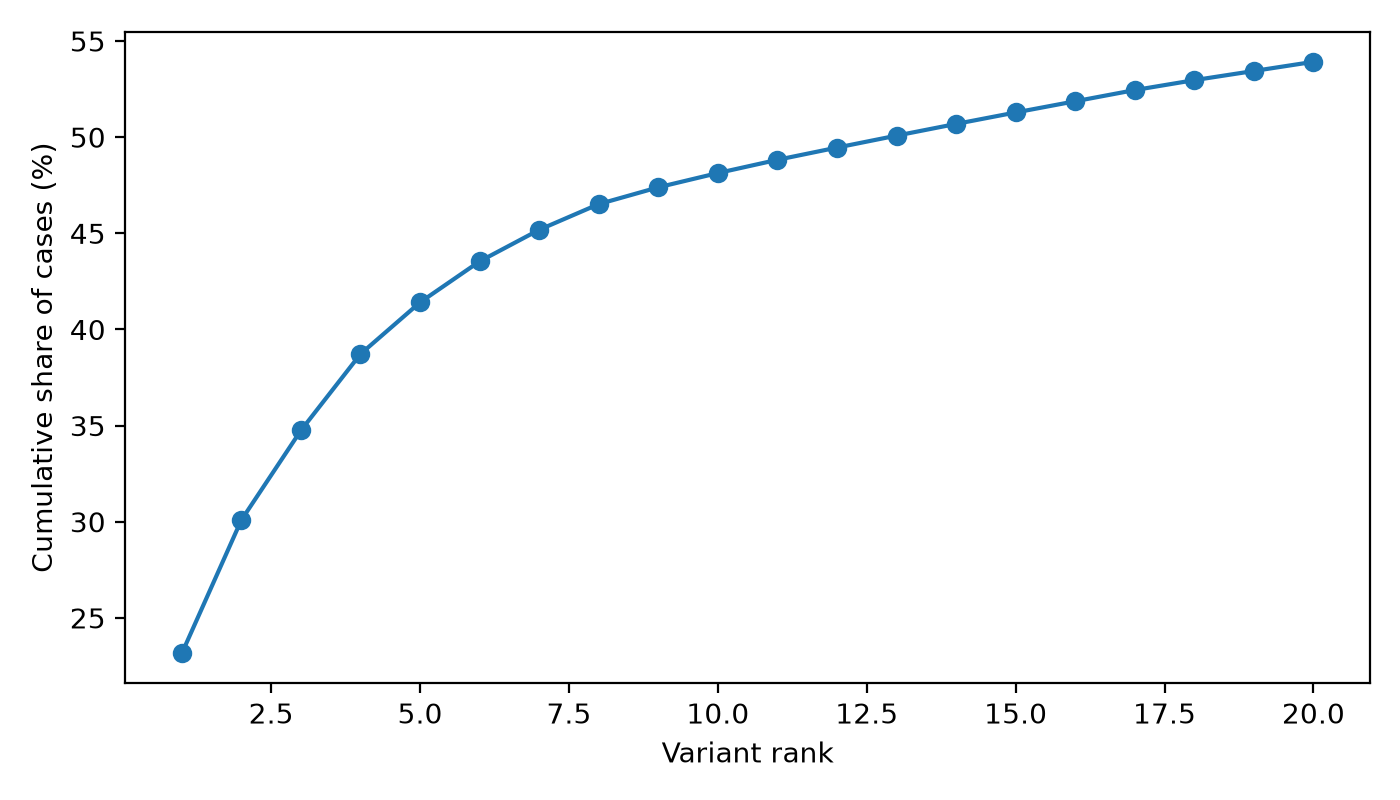
\includegraphics[width=\textwidth]{variant_pareto.png}
\end{column}
\begin{column}{0.46\textwidth}
Thousands of distinct variants against 7{,}554 cases.
\bigskip
Most variants occur exactly \emph{once}.
\bigskip
Consequence: any high-precision model of this log would be overfitted. The low
precision figures are the correct result.
\end{column}
\end{columns}
\end{frame}

\section{Verification}


\begin{frame}{The property library}
Eight properties, each a real formula evaluated per case.
\bigskip
\small
\begin{tabular}{ll}
\toprule
Termination & $\mathbf{F}(\textit{completed}_*)$ \\
Resolution & $\mathbf{G}(\textit{in\_progress} \rightarrow \mathbf{F}\,\textit{completed}_*)$ \\
No work after closure & $\mathbf{G}(\textit{closed} \rightarrow \neg\mathbf{F}\,\textit{in\_progress})$ \\
Queued work picked up & $\mathbf{G}(\textit{queued} \rightarrow \mathbf{F}\,\textit{in\_progress})$ \\
\alert{Formal closure} & $\mathbf{G}(\textit{in\_progress} \rightarrow \mathbf{F}\,\textit{closed})$ \\
\alert{Queueing precedes work} & $(\neg\,\textit{in\_progress}) \ \mathbf{U}\ \textit{queued}$ \\
\bottomrule
\end{tabular}
\bigskip\normalsize

The last two encode the \emph{documented} procedure. They are expected to fail.
The size of the gap is the result.
\end{frame}

\begin{frame}{Verification results}
\begin{center}\small\begin{tabular}{lrrr}
\toprule
Property & Satisfied & Violated & Ratio \\
\midrule
Termination & 7,546 & 8 & 0.999 \\
Resolution & 7,545 & 9 & 0.999 \\
No work after closure & 7,435 & 119 & 0.984 \\
Queued work is picked up & 7,494 & 60 & 0.992 \\
Waiting on the user resumes & 7,550 & 4 & 0.999 \\
No unmatched events & 7,549 & 5 & 0.999 \\
Formal closure & 5,591 & 1,963 & 0.740 \\
Queueing precedes work & 1,168 & 6,386 & 0.155 \\
\bottomrule
\end{tabular}
\end{center}
\vspace{-0.3em}
\begin{center}
\small Every case of the incident log, every property. No sampling.
\end{center}
\end{frame}


\section{Findings}

\begin{frame}{Finding 1: rework dominates}
\begin{center}
\Large
Fewer than half of all events are the \emph{first} occurrence\\
of their activity within the case.
\end{center}
\bigskip
\begin{itemize}
  \item Over half of all recorded work is repetition.
  \item Completion is near perfect; variability is moderate.
  \item Rework is the single component dragging the composite score down,
        and the largest available lever.
\end{itemize}
\end{frame}


\begin{frame}{Finding 2: push to front}
\begin{center}
\Large
$(\neg\,\textit{in\_progress}) \ \mathbf{U}\ \textit{queued}$ \quad holds for a
small minority of cases.
\end{center}
\bigskip
\begin{itemize}
  \item The documented procedure: queue the incident, then work it.
  \item What happens: work begins without the incident ever being queued.
  \item Established by \emph{formal verification over every case}, not by
        sampling, not by eyeballing variants.
\end{itemize}
\end{frame}




\section{Implementation}

\begin{frame}{Four layers, no state between them}
\begin{columns}[T]
\begin{column}{0.5\textwidth}
\textbf{The packages}
\begin{description}
  \item[\texttt{logs}] loading, schema detection, filters
  \item[\texttt{mining}] discovery, conformance, performance
  \item[\texttt{verification}] temporal logic per trace
  \item[\texttt{analysis}] score, anomalies, prediction
\end{description}
\smallskip
\texttt{ui}, \texttt{reporting} and \texttt{scripts} sit on top; nothing depends
on \texttt{ui}.
\end{column}
\begin{column}{0.46\textwidth}
\textbf{Consequences}
\begin{itemize}
  \item Every function takes a loaded log and returns a value: no module
        state, no cache
  \item Dashboard callbacks are plain functions, called directly by 211 tests
  \item Two browser sessions are independent
  \item Every table and figure on these slides is generated from code
\end{itemize}
\end{column}
\end{columns}
\end{frame}


\begin{frame}{It is one application, not a folder of scripts}
Everything shown in this talk is reachable from a single Gradio dashboard,
started with one command:
\bigskip
\begin{center}
\texttt{uv run python -m volvo.main}
\end{center}
\bigskip
\begin{columns}[T]
\begin{column}{0.48\textwidth}
\textbf{Eight tabs}
\begin{description}
  \item[Data] load a log, choose the activity label
  \item[Preprocessing] filters, deduplication
  \item[Discovery] miner, threshold, Petri net
  \item[Conformance] the four dimensions
\end{description}
\end{column}
\begin{column}{0.48\textwidth}
\textbf{\phantom{Eight tabs}}
\begin{description}
  \item[LTL] the shipped properties, or your own
  \item[Analytics] waiting times, variants, score
  \item[Report] the document, generated
  \item[Assistant] questions in natural language
\end{description}
\end{column}
\end{columns}
\end{frame}

\begin{frame}{What the dashboard lets you do}
\begin{itemize}
  \item \textbf{Change the labelling and rediscover.} The \act{Status} against
        \act{Status+Sub Status} comparison is two clicks, not two scripts.
  \item \textbf{Type a formula.} The LTL box accepts an arbitrary
        temporal-logic property over the activity alphabet and evaluates it
        against every case, returning violating cases as counterexamples. The
        eight shipped properties use that same code path.
  \item \textbf{Swap the miner and the threshold} and watch precision and net
        size move together.
  \item \textbf{Generate the report} and ask the assistant about the loaded log,
        with OpenAI, Gemini or a local Ollama model, or none at all.
\end{itemize}
\bigskip
State lives per browser session, so two people using it do not collide.
\end{frame}

\begin{frame}{Threats to validity}
\begin{itemize}
  \item Conformance is computed on a \emph{sample}; alignment-based computation
        does not scale to the full log.
  \item Token-based replay is optimistic on unsound nets. Alignments agree on
        the sample.
  \item The composite score's weights are \emph{stipulated}. Components are
        meaningful; the aggregate only comparatively.
  \item \act{Unmatched+Unmatched} is an export artefact, not work. Retained so
        its prevalence is visible.
  \item We observe what was \emph{recorded}. Poor recording discipline looks
        like rework.
\end{itemize}
\end{frame}

\begin{frame}{Conclusions}
\begin{enumerate}
  \item \textbf{Rework dominates}: over half of recorded work is repetition.
  \item \textbf{Documented $\neq$ executed}: push-to-front proved formally
        over every case.
  \item \textbf{Alpha is inapplicable here}: predicted by length-one loops,
        not an empirical surprise.
\end{enumerate}
\bigskip
\textbf{Next:} the organisational attributes are already loaded. Handover
analysis across support lines, push-to-front quantified by organisation, and
incident versus problem as interacting processes.
\end{frame}

\begin{frame}[plain]
\begin{center}
\Huge Questions
\end{center}
\end{frame}

\end{document}
